\documentclass[final,hyperref={pdfpagelabels=false}]{beamer}
\usepackage{grffile}
\mode<presentation>{\usetheme{I6pd2}}
\usepackage[english]{babel}
\usepackage[latin1]{inputenc}
\usepackage{amsmath,amsthm, amssymb, latexsym}
\usepackage{multirow}
\usepackage{xcolor}
%\usepackage{times}\usefonttheme{professionalfonts}  % obsolete
%\usefonttheme[onlymath]{serif}
\boldmath
\usepackage[orientation=portrait,size=a0,scale=1.4,debug]{beamerposter}
% change list indention level
% \setdefaultleftmargin{3em}{}{}{}{}{}

\newcommand{\GeV}{\textsf{GeV}}

%\usepackage{snapshot} % will write a .dep file with all dependencies, allows for easy bundling

\usepackage{array,booktabs,tabularx}
\newcolumntype{Z}{>{\centering\arraybackslash}X} % centered tabularx columns
\newcommand{\pphantom}{\textcolor{ta3aluminium}} % phantom introduces a vertical space in p formatted table columns??!!

\listfiles

%%%%%%%%%%%%%%%%%%%%%%%%%%%%%%%%%%%%%%%%%%%%%%%%%%%%%%%%%%%%%%%%%%%%%%%%%%%%%%%%%%%%%%
\graphicspath{{figures/}}
 
\title{Low-latency L1 Trigger Inference using GNN for $\tau \rightarrow 3 \mu$}
\author{
	Hyeon-Seo Yun{\color{lightgray}\inst{1}}, \href{https://mia.physics.purdue.edu/}{Mia Liu}{\color{lightgray}\inst{1}}
}
\institute{\color{lightgray}\inst{1} Purdue University \inst{2} Fermilab \inst{3} MIT
  \inst{4} CERN \inst{5} UW \inst{6} UIC \inst{7} HawkEye360}
\date[November 16, 2022]{November 16, 2022}




%%%%%%%%%%%%%%%%%%%%%%%%%%%%%%%%%%%%%%%%%%%%%%%%%%%%%%%%%%%%%%%%%%%%%%%%%%%%%%%%%%%%%%
\newlength{\columnheight}
\setlength{\columnheight}{105cm}

\newcommand{\hlsfml}{{\href{https://github.com/hls-fpga-machine-learning/hls4ml}{\texttt{hls4ml}}}}

%%%%%%%%%%%%%%%%%%%%%%%%%%%%%%%%%%%%%%%%%%%%%%%%%%%%%%%%%%%%%%%%%%%%%%%%%%%%%%%%%%%%%%
\begin{document}
\begin{frame}
  \begin{columns}
    % ---------------------------------------------------------%
    % Set up a column 
    \begin{column}{.49\textwidth}
      \begin{beamercolorbox}[center,wd=\textwidth]{postercolumn}
        \begin{minipage}[T]{.95\textwidth}  % tweaks the width, makes a new \textwidth
          \parbox[t][\columnheight]{\textwidth}{ % must be some better way to set the the height, width and textwidth simultaneously
            % Since all columns are the same length, it is all nice and tidy.  You have to get the height empirically
            % ---------------------------------------------------------%
            % fill each column with content
            
            \begin{block}{Need for low-latency in L1 Trigger}
                  \begin{center}
                    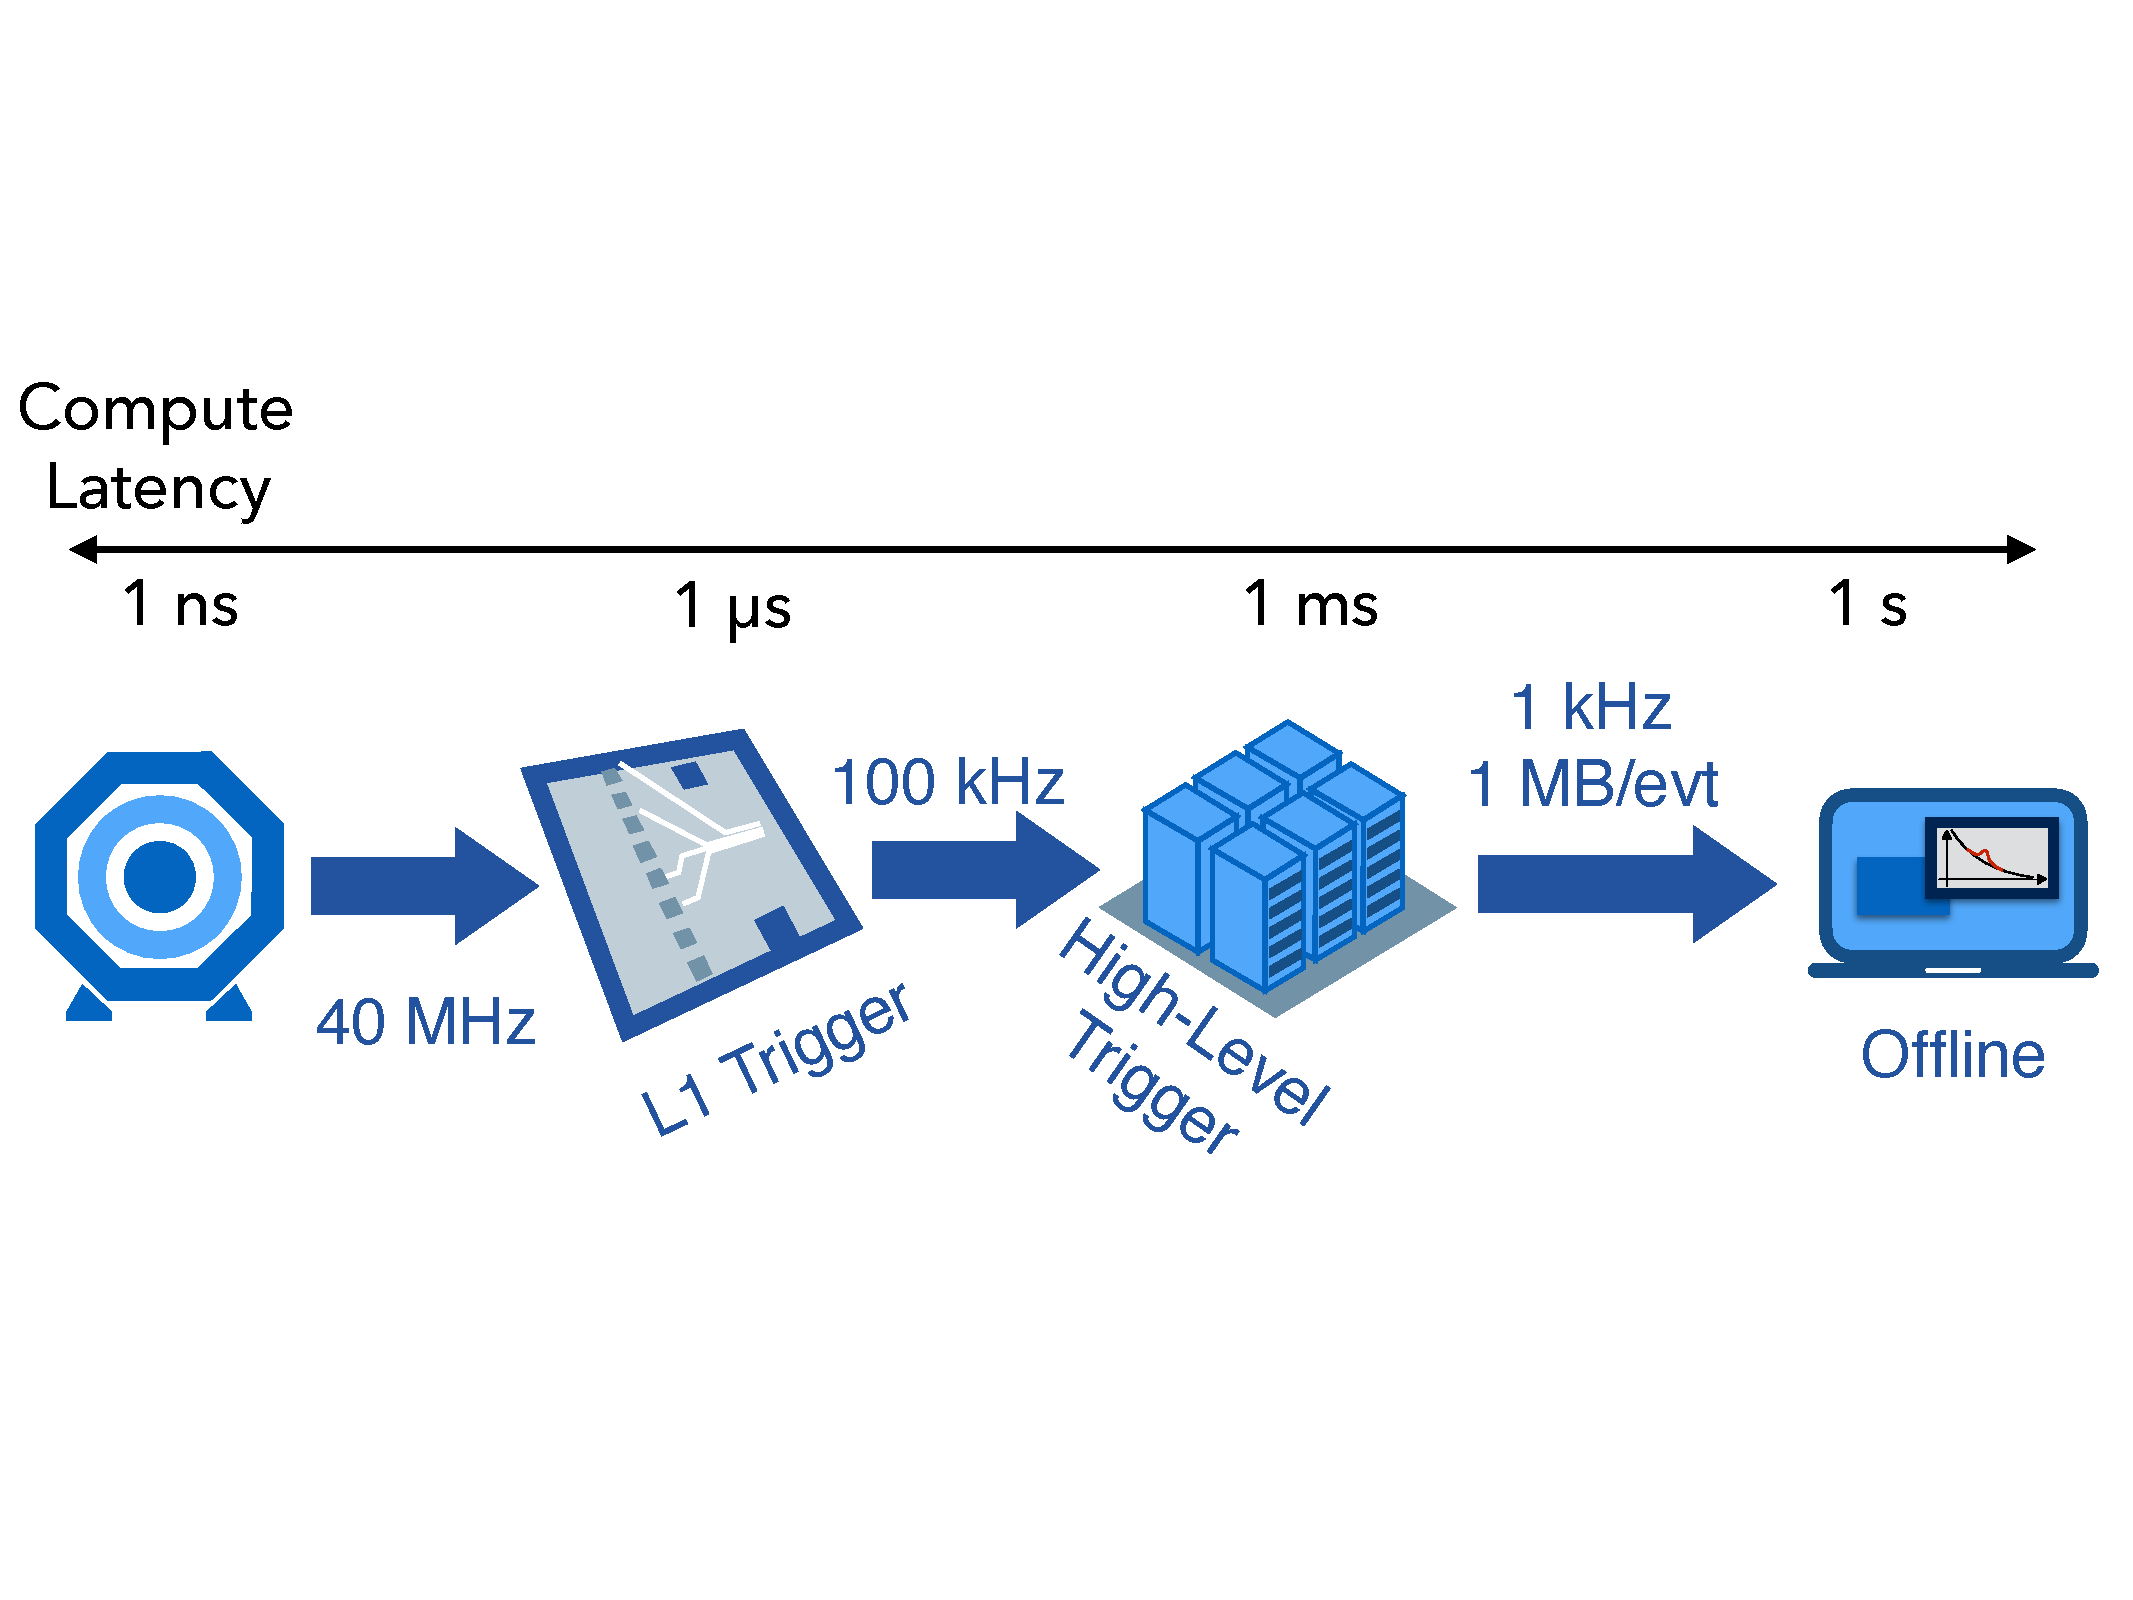
\includegraphics[viewport=0 200 1024 600, clip=true,width=\linewidth]{figures/cms_dataflow.pdf}
                  \end{center}
                  \begin{itemize}
                    \item Machine learning (ML) use case in particle physics: L1 Trigger, thge first stage of real-time data processing and
                      filtering, using field programmable gate arrays (FPGAs)
                    \item CERN CMS L1 Trigger requirements: high input data rates $>100$ TB/s,
                      $<100$ns fixed algorithm latency, constrained FPGA resources
                    \item Compiler based on high-level synthesis (HLS) called \hlsfml~to rapidly prototype ML models in FPGAs
              \end{itemize}
            \end{block}

            \begin{block}{Usage of Graph Neural Networks (GNN) in Filtering Task}
              \begin{itemize}
              \item Task: differentiate showers (or \emph{jets})
                produced in decays of heavy standard model
                particles ($W$ and $Z$ bosons and top quarks),
                from backgrounds consisting mainly of light quark-
                ($u$, $d$, $c$, $s$, $b$) and gluon-initiated jets 
                \end{itemize}
              \begin{columns}              
              \begin{column}{.49\textwidth}
                \begin{itemize}
              \item GNN
              \item Performance quantified in a receiver operating
                characteristic (ROC) curve of signal efficiency versus
                misidentification rate for quark, gluon, $W$ boson,
                $Z$ boson, and top quark jets
              \end{itemize}
            \end{column}
            \begin{column}{.49\textwidth}
             \begin{center}
                    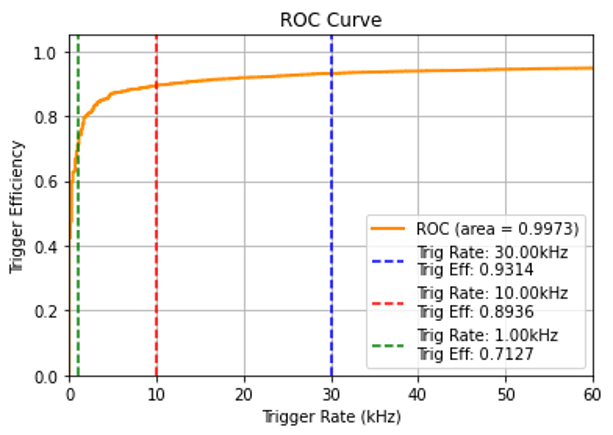
\includegraphics[width=\linewidth]{gnn_roc.png}
                  \end{center}
                \end{column}
                \end{columns}
              \end{block}
            \begin{block}{Design}
                  \begin{center}
                    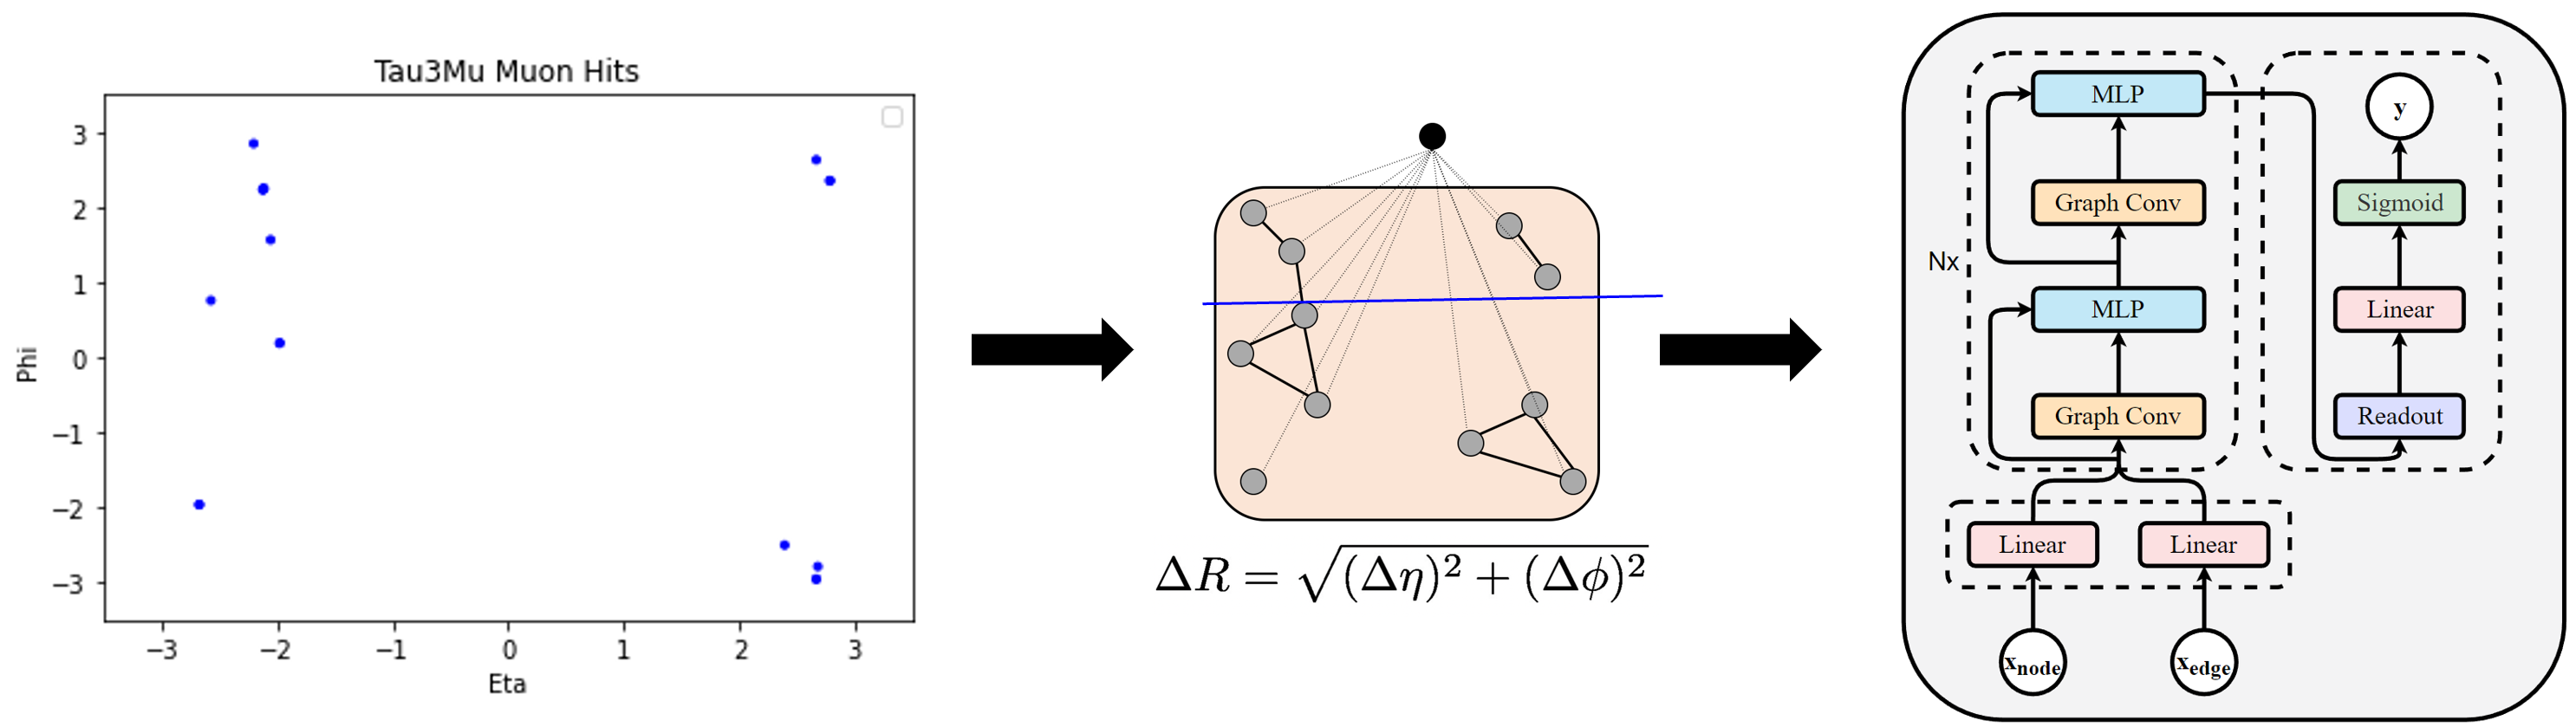
\includegraphics[width=\linewidth]{figures/graph_creation.png}
                  \end{center}
                \vspace{0.5in}
                Explore the FPGA design space through
                \begin{itemize}
                \item {\bf compression}, the three-hidden-layer model with 70\% of the parameters removed using iterative retraining with $L_1$ regularization and magnitude-based pruning
                \item {\bf quantization}, the precision of the inputs, weights, and biases
                \item {\bf parallelization}, the number of times a
                  given multiplier is used for a layer computation,
                  quantified by a \emph{reuse factor}
                \end{itemize}
                \vspace{0.5in}
                With these handles, monitor 
                \begin{itemize}
                \item {\bf resources}: digital signal processors
                  (DSPs), block random access memory (BRAM), flip-flops (FFs), and lookup tables (LUTs)
                \item {\bf latency}: time it takes to compute the full network
                \item {\bf initiation interval (II)}: time before a new set of inputs can be accepted
                \end{itemize}
              \end{block}
              
                }
              \end{minipage}
            \end{beamercolorbox}
          \end{column}
    % ---------------------------------------------------------%
    % end the column

    % ---------------------------------------------------------%
    % Set up a column 
    \begin{column}{.49\textwidth}
      \begin{beamercolorbox}[center,wd=\textwidth]{postercolumn}
        \begin{minipage}[T]{.95\textwidth} 
          \parbox[t][\columnheight]{\textwidth}{
            
            \begin{block}{FPGA Implementation via hls4ml}
             \begin{center}
                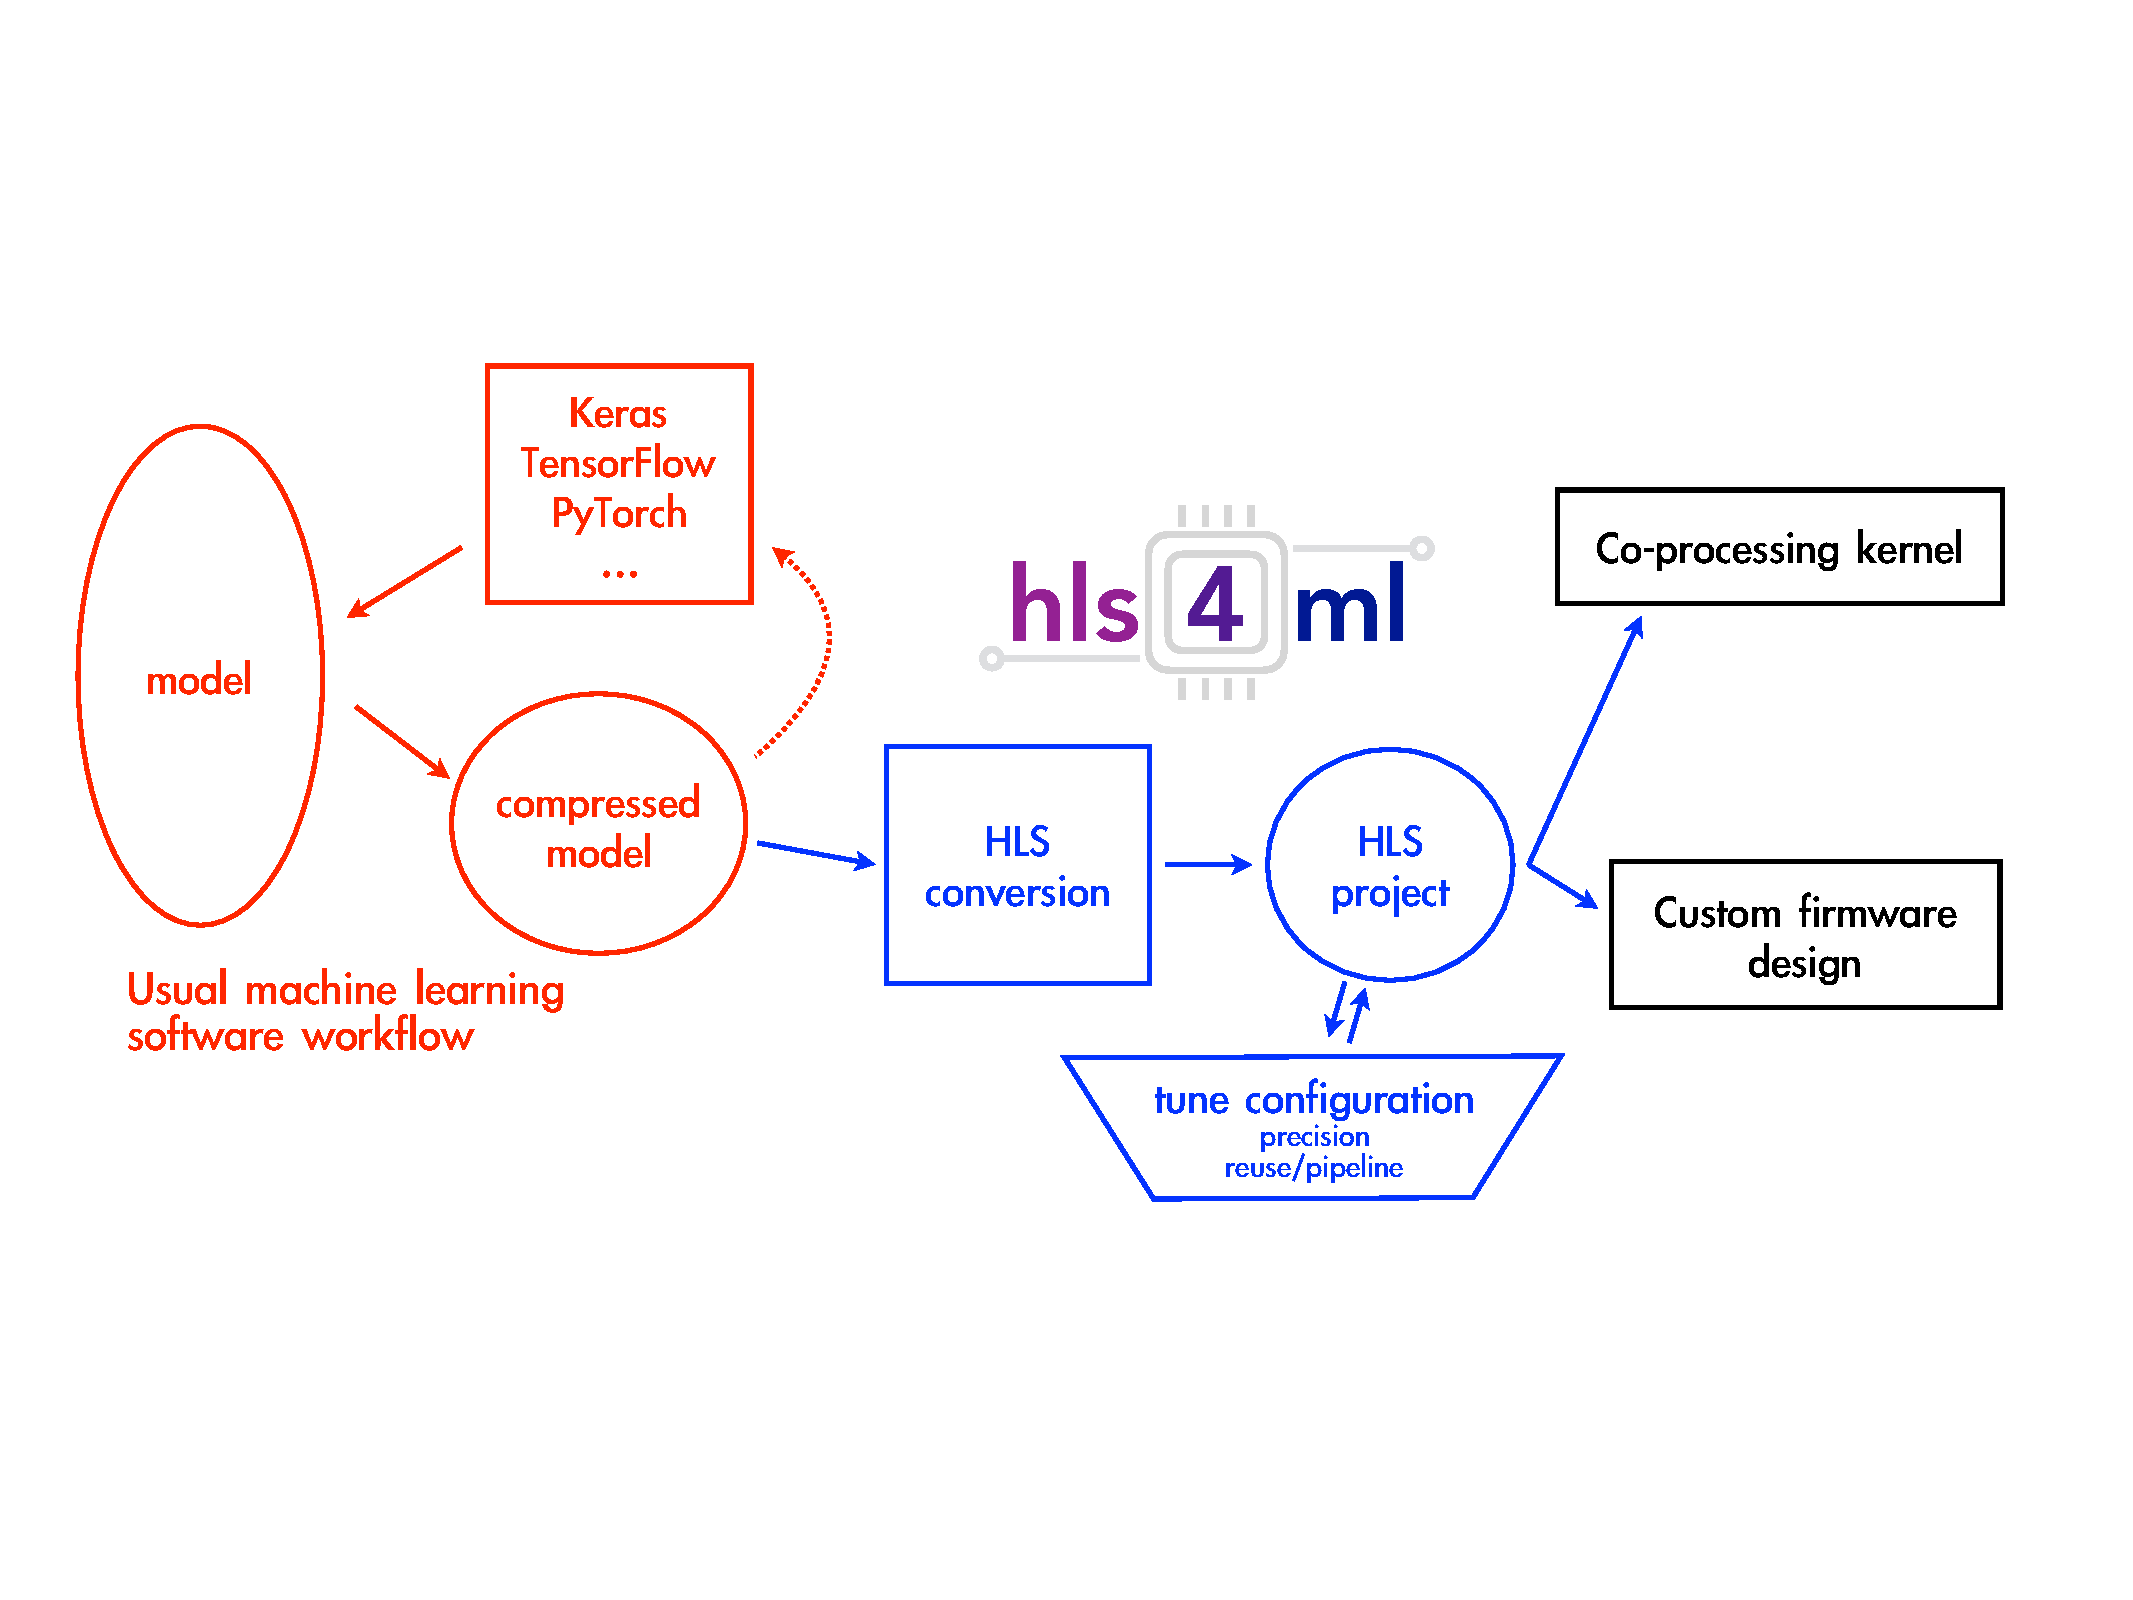
\includegraphics[width=0.8\linewidth]{flow-hls4ml.pdf}
              \end{center}
              \begin{itemize}
                \item First evaluate NN with fixed point precision:
                  {\tt <16,6>} fixed-point precision reproduces the
                  ROC curve performance
                \item DSP usage in the compressed 3-hidden-layer model
                  increases as a function of the network precision and
                  decreases for larger reuse factors
                  \item Latency increases from 10 to 35 clock cycles
                    (50 to 175~ns) for larger reuse factors
                  \item Results based on Xilinx Kintex Ultrascale FPGA part number
                    \texttt{xcku115-flvb2104-2-i}, 200~MHz clock
                    frequency, Vivado HLS 2017.2
              \end{itemize}
             
            \end{block}
                  \begin{block}{Quantization Aware Training}
                    To enhance the flexibility of \hlsfml, several new
                    developments include
                    \begin{itemize}
                    \item extension to allow for
                      significantly larger dense networks in terms of the number of neurons per layer
                    \item inclusion of zero-suppression for weights
                      stored in on-chip memory or BRAM, reducing the use of on-chip logic registers
                    \item addition of binary and ternary matrix multiplication
                    \end{itemize}
                \vspace{0.5in}
                    To demonstrate the new developments, several versions of a large dense network to classify handwritten MNIST digits are benchmarked
                    \begin{center}
                    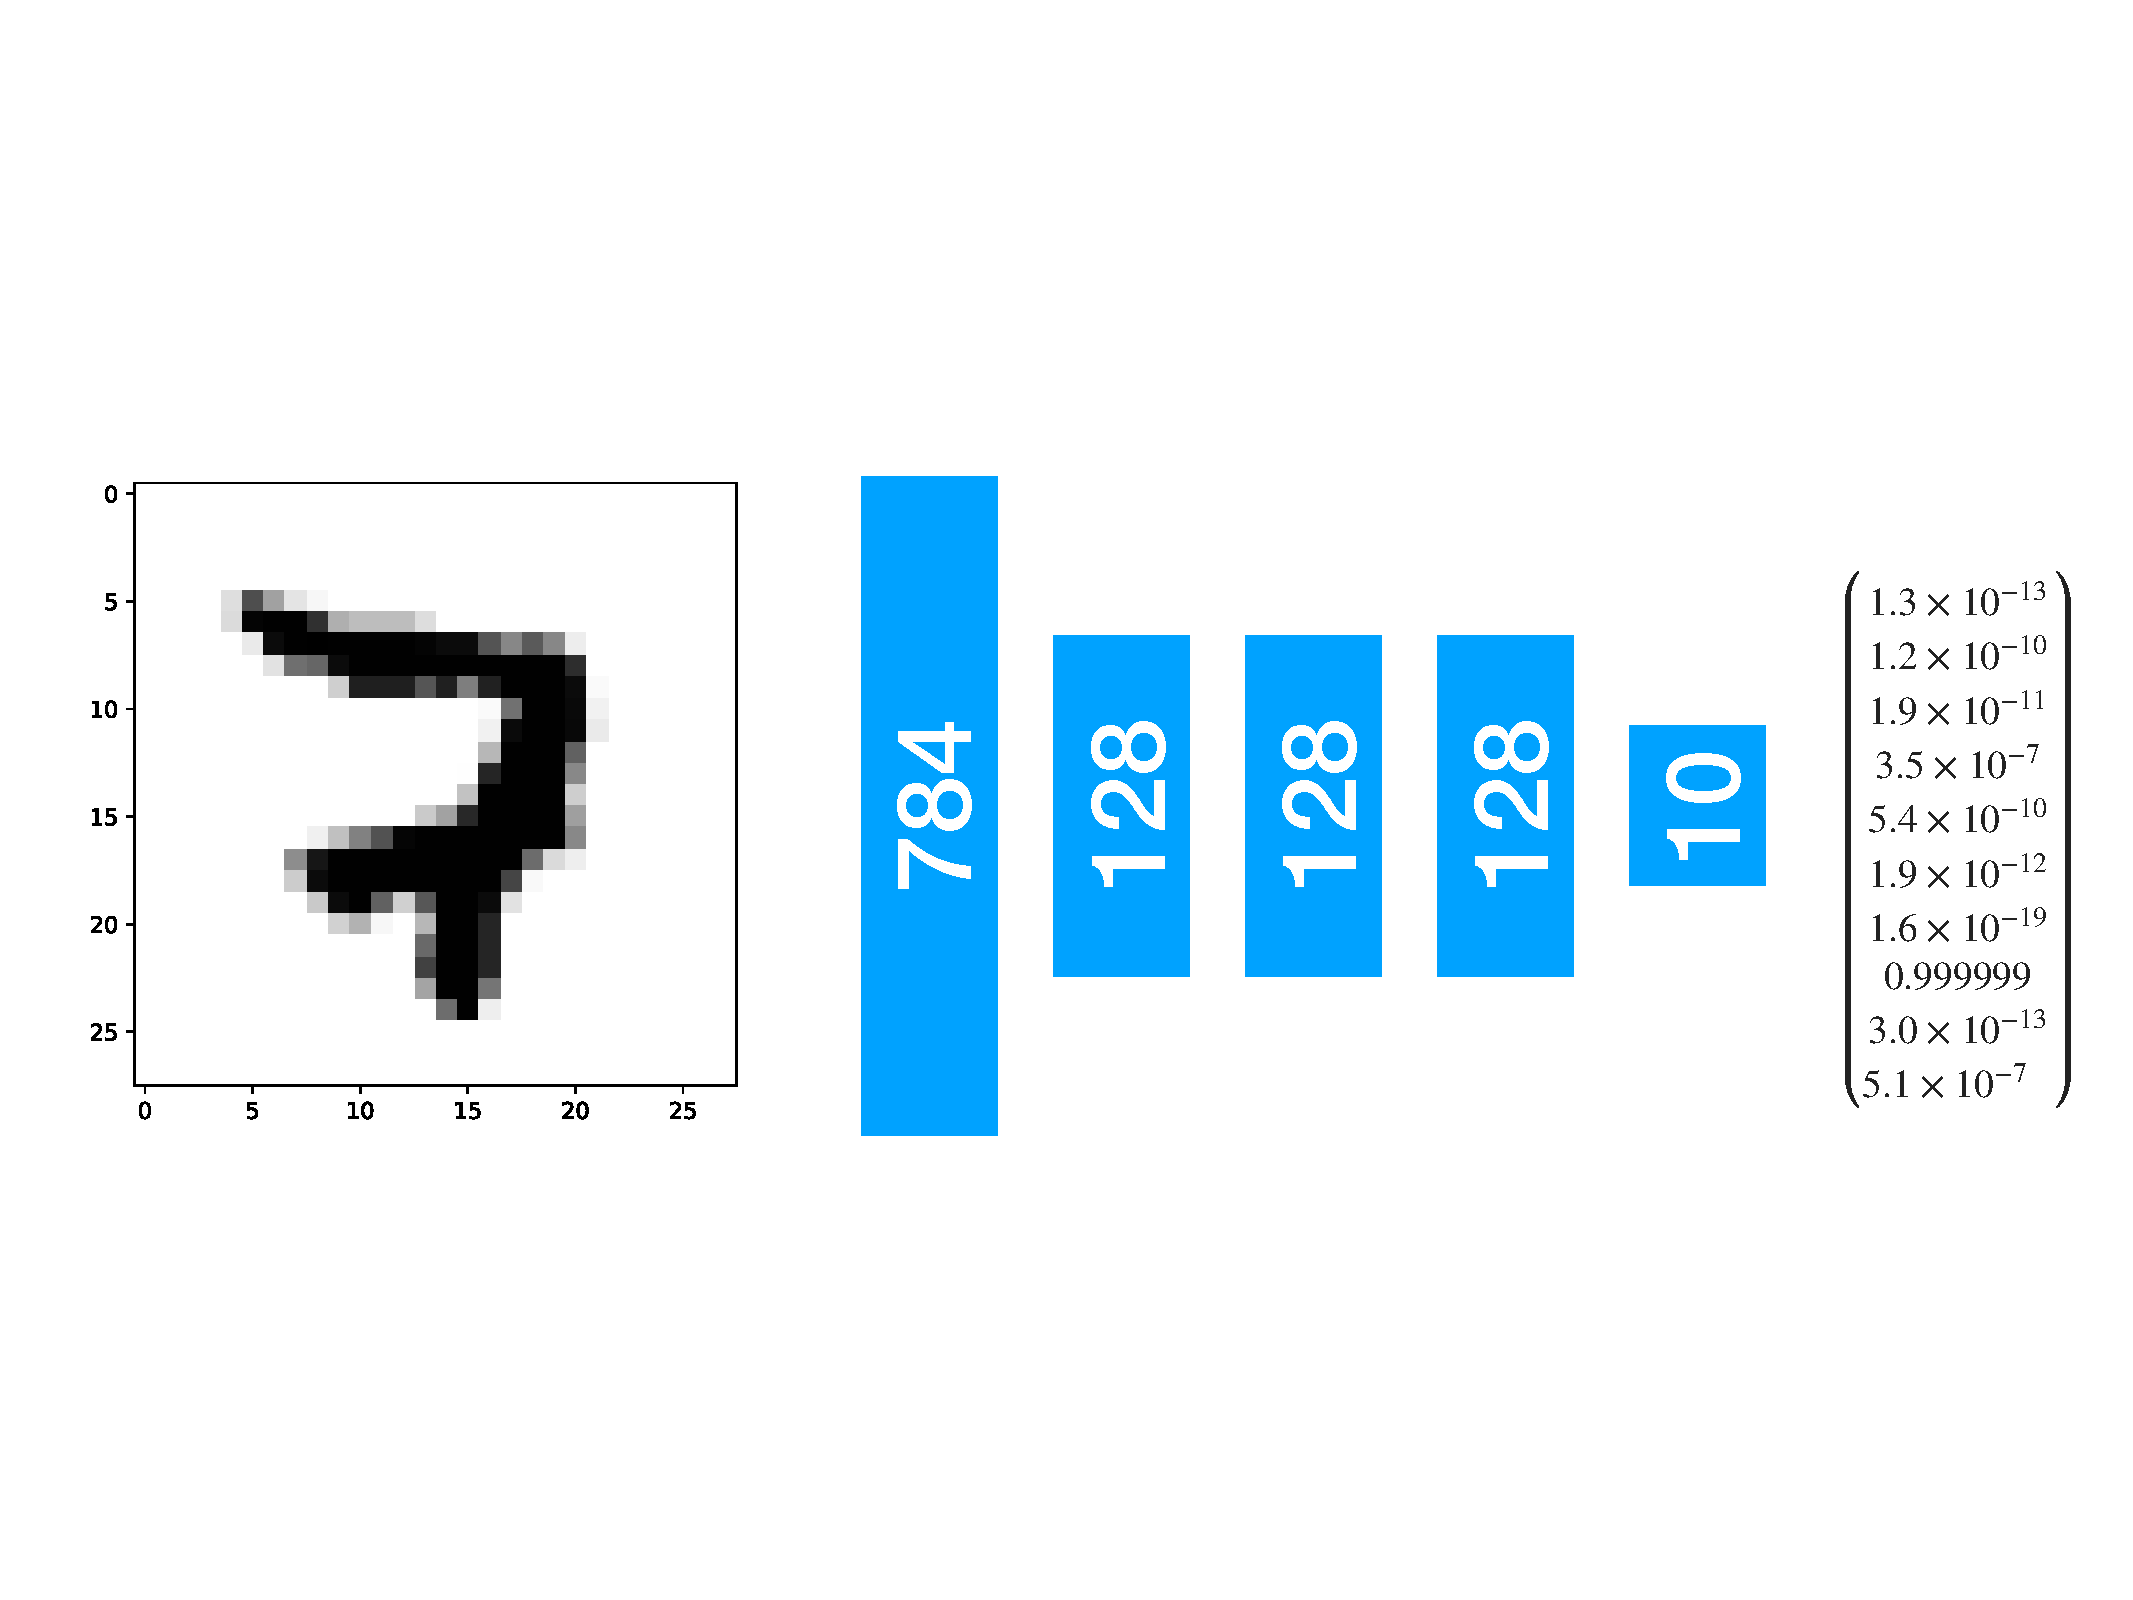
\includegraphics[width=\linewidth]{MNIST_big.pdf}
                  \end{center}
                  \begin{center}
                    \resizebox{\textwidth}{!}{
                      \begin{tabular}{l|ccccccc}
                        \textbf{Model} & \textbf{II} & \textbf{Accuracy} &\textbf{Latency} & \textbf{DSP}  & \textbf{BRAM} & \textbf{FF}  & \textbf{LUT}\\\hline
                        MNIST dense                                            &  128 & 0.97 & 2.6~$\mu$s & 21\% & 45\%& 12\% & 33\%\\
                        MNIST binary dense                                 &  128 & 0.93 & 2.6~$\mu$s & 0\% & 33\%& 7\% & 39\%\\ 
                        MNIST ternary dense                                &  128 & 0.95 & 2.6~$\mu$s & 0\% & 33\%& 7\% & 40\%\\ 
                        MNIST dense, 95\% pruned &  128 & 0.96 & 2.8~$\mu$s & 1\% & 34\% & 13\% & 164\%\\
                        MNIST dense                       &  4096 & 0.97 & 68.1~$\mu$s &1\% & 66\%&27\% &83\%\\ 
                        MNIST dense, 95\% pruned &  4096 & 0.96 & 82.1~$\mu$s & 0\% & 34\% & 9\% & 25\%\\ 
                      \end{tabular}}                       
                  \end{center}
                \end{block}                
                \begin{block}{Summary}
                  \begin{itemize}
                    \item \hlsfml: compiler based on HLS for porting
                      fully-connected NNs to an FPGA from
                      conventional training frameworks such as {\tt
                        Keras} and {\tt PyTorch}
                      \item Focus on real-time
                        event reconstruction and filtering at the LHC
                        in FPGAs, with many other applications to real-time detector systems in the physical
                        sciences 
                        \item  Implemented a dense 3-hidden-layer NN
                          in a Xilinx Kintex Ultrascale using roughly
                          10\% of the available DSPs and latency of
                          approximately 75--150~ns with a clock
                          frequency of 200~MHz 
                          \item Extend the capabilities and
                            flexibility of \hlsfml~to allow larger
                            NN architectures for applications with
                            latency constraints of approximately 1--100~$\mu$s 
                          \end{itemize}
                          \begin{flushright}\vspace{-3ex}
                           % \href{https://ml4physicalsciences.github.io/files/NeurIPS_ML4PS_2019_74.pdf}{
\includegraphics[width=0.18\textwidth]{qrcode.png}}
                          \end{flushright}
                  \end{block}                  
          }
          % ---------------------------------------------------------%
          % end the column
        \end{minipage}
      \end{beamercolorbox}
    \end{column}
    % ---------------------------------------------------------%
    % end the column
  \end{columns}
  \vskip1ex
  %\tiny\hfill\textcolor{ta2gray}{Created with \LaTeX \texttt{beamerposter}  \url{http://www-i6.informatik.rwth-aachen.de/~dreuw/latexbeamerposter.php}}
  %\tiny\hfill{Created with \LaTeX \texttt{beamerposter}  \url{http://www-i6.informatik.rwth-aachen.de/~dreuw/latexbeamerposter.php} \hskip1em}
\end{frame}
\end{document}


%%%%%%%%%%%%%%%%%%%%%%%%%%%%%%%%%%%%%%%%%%%%%%%%%%%%%%%%%%%%%%%%%%%%%%%%%%%%%%%%%%%%%%%%%%%%%%%%%%%%
%%% Local Variables: 
%%% mode: latex
%%% TeX-PDF-mode: t
%%% Comments below:



\href{https://jduarte.physics.ucsd.edu}{Javier Duarte}{\color{lightgray}\inst{1,2}},  Christian Herwig{\color{lightgray}\inst{2}},
	  Burt Holzman{\color{lightgray}\inst{2}}, Sergo Jindariani{\color{lightgray}\inst{2}}, Benjamin
	  Kreis{\color{lightgray}\inst{2}},  \href{https://mia.physics.purdue.edu/}{Mia Liu}{\color{lightgray}\inst{2}}, Ryan
	  Rivera{\color{lightgray}\inst{2}},  Nhan Tran{\color{lightgray}\inst{2}},  Song Han{\color{lightgray}\inst{3}},  Phil
	  Harris{\color{lightgray}\inst{3}},  Dylan Rankin{\color{lightgray}\inst{3}}, Vladimir Loncar{\color{lightgray}\inst{4}},
	  Jennifer Ngadiuba{\color{lightgray}\inst{4}}, Maurizio Pierini{\color{lightgray}\inst{4}}, Sioni
	  Summers{\color{lightgray}\inst{4}}, Scott Hauck{\color{lightgray}\inst{5}}, Shih-Chieh Hsu{\color{lightgray}\inst{5}}, Zhenbin Wu{\color{lightgray}\inst{6}},  Edward 	Kreinar{\color{lightgray}\inst{7}}

